\documentclass[12pt]{article}
\usepackage{amsmath}
\usepackage{graphicx}
\usepackage{hyperref}
\usepackage{listings}
\usepackage{color}
\usepackage{pythonhighlight}

\title{Operating System Course Report - First Half of the Semester}
\author{A class}
\date{\today}

\begin{document}

\maketitle
\newpage

\tableofcontents
\newpage

\section{Introduction}
This report summarizes the topics covered during the first half of the Operating System course. It includes theoretical concepts, practical implementations, and assignments. The course focuses on the fundamentals of operating systems, including system architecture, process management, CPU scheduling, and deadlock handling.

\section{Course Overview}
\subsection{Objectives}
The main objectives of this course are:
\begin{itemize}
    \item To understand the basic components and architecture of a computer system.
    \item To learn process management, scheduling, and inter-process communication.
    \item To explore file systems, input/output management, and virtualization.
    \item To study the prevention and handling of deadlocks in operating systems.
\end{itemize}

\subsection{Course Structure}
The course is divided into two halves. This report focuses on the first half, which covers:
\begin{itemize}
    \item Basic Concepts and Components of Computer Systems
    \item System Performance and Metrics
    \item System Architecture of Computer Systems
    \item Process Description and Control
    \item Scheduling Algorithms
    \item Process Creation and Termination
    \item Introduction to Threads
    \item File Systems
    \item Input and Output Management
    \item Deadlock Introduction and Prevention
    \item User Interface Management
    \item Virtualization in Operating Systems
\end{itemize}

\section{Topics Covered}

\subsection{Basic Concepts and Components of Computer Systems}
This section explains the fundamental components that make up a computer system, including the CPU, memory, storage, and input/output devices.

\subsection{System Performance and Metrics}
This section introduces various system performance metrics used to measure the efficiency of a computer system, including throughput, response time, and utilization.

\subsection{System Architecture of Computer Systems}
Describes the architecture of modern computer systems, focusing on the interaction between hardware and the operating system.

\subsection{Process Description and Control}
Processes are a central concept in operating systems. This section covers:
\begin{itemize}
    \item Process states and state transitions
    \item Process control block (PCB)
    \item Context switching
\end{itemize}

\subsection{Scheduling Algorithms}

%Ilham Kurniawan - H071231024

\subsubsection{\textit{First-Come, First-Served} (FCFS)}

\begin{figure}[h]
    \centering
    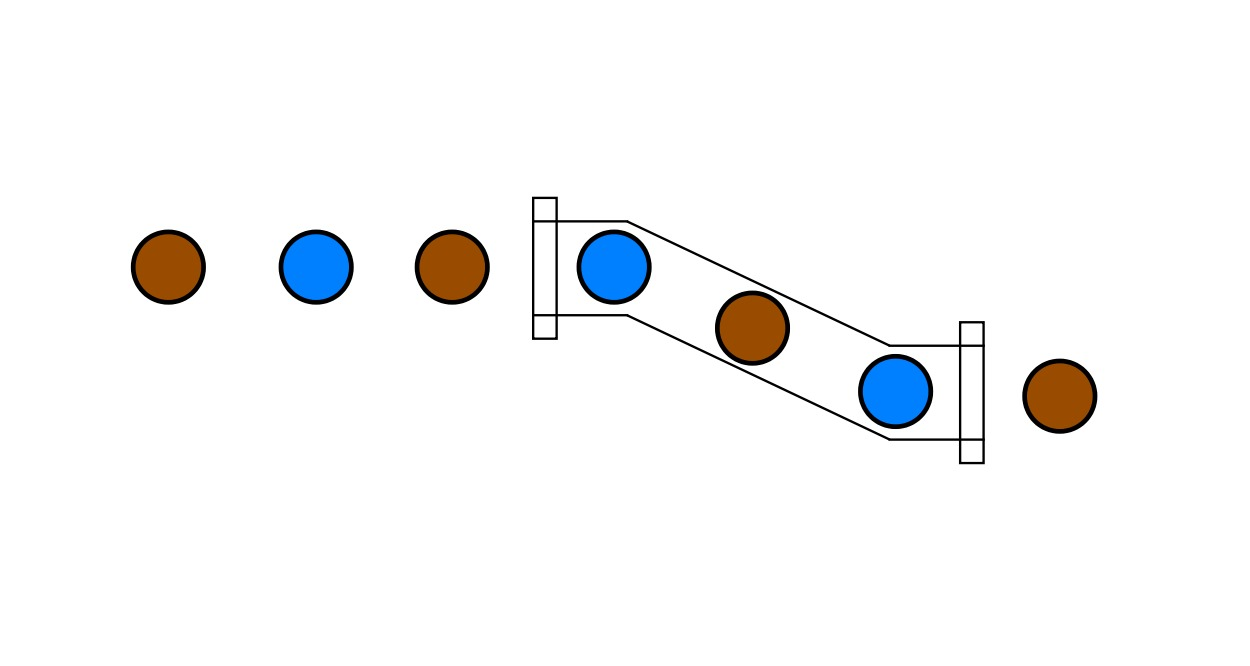
\includegraphics[width=0.9\textwidth]{asset/fcfs-illustration.jpg}
    \caption{Contoh ilustrasi algoritma FCFS.}
    \label{fig:contoh-ilustrasi-algoritma-fcfs}
\end{figure}

\hspace{1cm}

Algoritma \textbf{\textit{First-Come, First-Served} (FCFS)} atau \textbf{Pertama Datang, Pertama Dilayani} adalah salah satu metode penjadwalan paling sederhana yang digunakan dalam sistem operasi komputer, khususnya dalam alokasi waktu CPU. Prinsip dasar dari algoritma ini adalah bahwa setiap proses yang tiba lebih awal dalam keadaan \textit{ready} akan dimasukkan ke dalam antrian dengan prinsip \textit{First-In, First-Out} (FIFO). Proses yang tiba pertama kali akan mendapatkan jatah waktu CPU terlebih dahulu dan dieksekusi hingga selesai sebelum proses berikutnya dapat dilayani. Proses-proses lain yang datang setelahnya harus menunggu hingga proses sebelumnya selesai.


\hspace{1cm}

Dalam penerapannya pada penjadwalan CPU, metode FCFS menempatkan setiap proses dalam urutan waktu kedatangan, tanpa memperhitungkan berapa lama waktu yang diperlukan untuk mengeksekusi proses tersebut (\textit{burst time}). Artinya, proses dengan \textit{burst time} yang lebih panjang akan tetap dilayani terlebih dahulu jika datang lebih awal, meskipun hal ini dapat menyebabkan proses-proses lain yang lebih singkat harus menunggu lebih lama.

\hspace{1cm}

\textbf{Kelebihan dan Kekurangan FCFS}

\hspace{1cm}

\begin{itemize}
    \item \textbf{Kelebihan}:
\end{itemize}

\begin{enumerate}
    \item Sederhana dan mudah digunakan.
    \item \textit{Fair} karena tidak ada prioritas.
    \item Tidak ada \textit{starvation} karena setiap proses akan dijalankan jika sudah masuk ke antrian.
\end{enumerate}


\begin{itemize}
    \item \textbf{Kekurangan:}
\end{itemize}

\begin{enumerate}
    \item Kinerja yang buruk karena proses yang lebih singkat harus menunggu proses yang lebih lama selesai.
    \item Waktu tunggu umumnya tinggi.
    \item Tidak ideal untuk sistem waktu-berbagi karena tidak dapat memenuhi kebutuhan respons cepat.
\end{enumerate}

\renewcommand{\refname}{Sumber}
\begin{thebibliography}{}

\bibitem{guru99}
Guru99. (2023). \textit{First Come First Serve (FCFS) Scheduling Algorithm in OS}. Retrieved from \url{https://www.guru99.com/fcfs-scheduling.html}

\bibitem{scaler}
Scaler. (n.d.). \textit{First Come First Serve (FCFS) Scheduling Algorithm}. Retrieved October 10, 2024, from \url{https://www.scaler.com/topics/first-come-first-serve/}

\bibitem{byjus}
BYJU'S. (n.d.). \textit{FCFS Scheduling - Full Form and Working}. Retrieved October 10, 2024, from \url{https://byjus.com/gate/fcfs-scheduling-full-form/}

\end{thebibliography}

\subsection{Process Creation and Termination}
Details how processes are created and terminated by the operating system, including:
\begin{itemize}
    \item Process spawning
    \item Process termination conditions
\end{itemize}

\subsection{Introduction to Threads}
This section introduces the concept of threads and their relation to processes, covering:
\begin{itemize}
    \item Single-threaded vs. multi-threaded processes
    \item Benefits of multithreading
\end{itemize}

\begin{figure}[h]
    \centering
    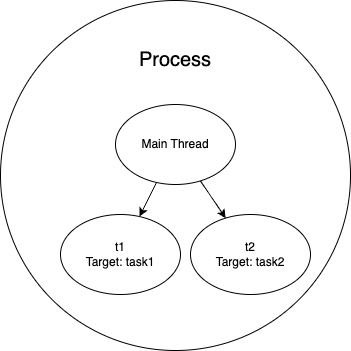
\includegraphics[width=0.5\textwidth]{/Users/khawaritzmi/Unhas/os_report_mid2024/a_class/asset/example.png}  % Sesuaikan nama file dan ukurannya
    \caption{Ini adalah gambar contoh dari multithreading.}
    \label{fig:contoh_gambar}
\end{figure}

Seperti yang terlihat pada Gambar \ref{fig:contoh_gambar}, inilah cara menambahkan gambar dengan keterangan.

\subsection{File Systems}
File systems provide a way for the operating system to store, retrieve, and manage data. This section explains:
\begin{itemize}
    \item File system structure
    \item File access methods
    \item Directory management
\end{itemize}

\subsection{Input and Output Management}
Input and output management is key for handling the interaction between the system and external devices. This section includes:
\begin{itemize}
    \item Device drivers
    \item I/O scheduling
\end{itemize}

\subsection{Deadlock Introduction and Prevention}
Explores the concept of deadlocks and methods for preventing them:
\begin{itemize}
    \item Deadlock conditions
    \item Deadlock prevention techniques
\end{itemize}

\subsection{User Interface Management}
This section discusses the role of the operating system in managing the user interface. Topics covered include:
\begin{itemize}
    \item Graphical User Interface (GUI)
    \item Command-Line Interface (CLI)
    \item Interaction between the user and the operating system
\end{itemize}

\subsection{Virtualization in Operating Systems}
Virtualization allows multiple operating systems to run concurrently on a single physical machine. This section explores:
\begin{itemize}
    \item Concept of virtualization
    \item Hypervisors and their types
    \item Benefits of virtualization in modern computing
\end{itemize}

\section{Assignments and Practical Work}
\subsection{Assignment 1: Process Scheduling}
Students were tasked with implementing various process scheduling algorithms (e.g., FCFS, SJN, and RR) and comparing their performance under different conditions.
\subsubsection{Group 1}
\begin{python}
    class Process:
    def __init__(self, pid, arrival_time, burst_time):
        self.pid = pid
        self.arrival_time = arrival_time
        self.burst_time = burst_time
        self.completion_time = 0
        self.turnaround_time = 0
        self.waiting_time = 0
\end{python}

\begin{table}[htbp] % Optional: For floating position
    \centering
    \begin{tabular}{|c|c|c|} % Defines number of columns and alignment (c = center, l = left, r = right). '|' creates vertical lines.
    \hline
    Header 1 & Header 2 & Header 3 \\ % Column headers
    \hline
    Row 1, Column 1 & Row 1, Column 2 & Row 1, Column 3 \\ % First row of data
    \hline
    Row 2, Column 1 & Row 2, Column 2 & Row 2, Column 3 \\ % Second row of data
    \hline
    \end{tabular}
    \caption{Your table caption} % Optional: For adding a caption
    \label{tab:your_label} % Optional: For cross-referencing the table
\end{table}
\subsection{Assignment 2: Deadlock Handling}
In this assignment, students were asked to simulate different deadlock scenarios and explore various prevention methods.

%Ilham Kurniawan - H071231024

\subsection{Assignment 3: Multithreading and Amdahl's Law}
\subsubsection{Pertanyaan dan Jawaban serta Implementasi Kode \textit{Python} untuk \textit{Multithreading and Amdahl’s Law}}

\textbf{Pertanyaan :} 

\vspace{0.2cm}

Mengapa fungsi thread.join() digunakan di dalam loop terakhir pada fungsi {contoh\_multithreading}

\begin{python}
Assignment 3

import threading
import time

def komputasi():
    # Simulasi tugas komputasi yang intensif
    time.sleep(1)  # Misalkan ini adalah pekerjaan yang memakan waktu

def contoh_multithreading(jumlah_thread):
    threads = []
    for _ in range(jumlah_thread):
        thread = threading.Thread(target=komputasi)
        threads.append(thread)
        thread.start()
    
    for thread in threads:
        thread.join()  # Tunggu semua thread selesai

# Menghitung percepatan menggunakan Hukum Amdahl
def hukum_amdahl(proporsi_sekuensial, jumlah_thread):
    proporsi_paralel = 1 - proporsi_sekuensial
    percepatan = 1 / (proporsi_sekuensial + (proporsi_paralel / jumlah_thread))
    return percepatan

# Asumsi proporsi pekerjaan yang tidak dapat diparalelkan
proporsi_sekuensial = 0.2  # 20% dari pekerjaan tidak dapat diparalelkan
jumlah_thread = 4
percepatan = hukum_amdahl(proporsi_sekuensial, jumlah_thread)
print(f"Percepatan teoritis dengan {jumlah_thread} thread: {percepatan}")
\end{python}

\textbf{Jawaban :} Fungsi thread.join() digunakan untuk memastikan bahwa program utama menunggu hingga setiap \textit{thread} selesai menjalankan tugasnya sebelum melanjutkan ke bagian kode berikutnya. Tanpa join(), program utama bisa saja berakhir lebih cepat atau menjalankan bagian kode berikutnya sebelum semua \textit{thread} selesai, yang bisa menyebabkan masalah dalam tugas yang bergantung pada hasil \textit{thread}.

%Ilham Kurniawan - H071231024

\subsection{Assignment 4: Simple Command-Line Interface (CLI) for User Interface Management}

\subsubsection{Pertanyaan dan Jawaban serta Implementasi Kode \textit{Python} untuk \textit{Command-Line Interface} (CLI) Sederhana}

\textbf{Pertanyaan} :

\vspace{0.2cm}

Jelaskan fungsi cli() dalam kode \textit{Python} di bawah dan sebutkan perintah-perintah apa saja yang didukung oleh CLI tersebut!

\begin{python}
Assignment 4

import os

def cli():
    while True:
        perintah = input("Masukkan perintah (buat, daftar, hapus, info, keluar): ")
        if perintah == "buat":
            nama_file = input("Masukkan nama file yang akan dibuat: ")
            open(nama_file, 'w').close()
            print(f"File {nama_file} telah dibuat.")
        elif perintah == "daftar":
            files = os.listdir('.')
            print("File:", files)
        elif perintah == "hapus":
            nama_file = input("Masukkan nama file yang akan dihapus: ")
            os.remove(nama_file)
            print(f"File {nama_file} telah dihapus.")
        elif perintah == "info":
            files = os.listdir('.')
            for file in files:
                if os.path.isfile(file):
                    print(f"File: {file}, Ukuran: {os.path.getsize(file)} bytes")
        elif perintah == "keluar":
            break
        else:
            print("Perintah tidak valid.")

cli()

\end{python}

\textbf{Jawaban} : Fungsi cli() dalam kode \textit{Python} tersebut merupakan antarmuka baris perintah sederhana yang memungkinkan \textit{user} untuk melakukan manipulasi \textit{file} dasar. Perintah yang didukung adalah:

\begin{itemize}
    \item buat: Membuat \textit{file} kosong dengan nama yang diberikan oleh \textit{user}.
    \item daftar: Menampilkan semua \textit{file} yang ada di direktori saat ini.
    \item hapus: Menghapus \textit{file} dengan nama yang diberikan oleh \textit{user}.
    \item keluar: Mengakhiri program CLI.
\end{itemize}

%Ilham Kurniawan - H071231024

\subsection{Assignment 5: File System Access}
\subsubsection{Pertanyaan dan Jawaban serta Implementasi Kode \textit{Python} untuk File\textit{ System Access}}

\textbf{Pertanyaan :}

\vspace{0.2cm}

Jelaskan bagaimana cara membuat \textit{file} baru dan menulis konten ke \textit{file} tersebut di dalam kode di bawah!

\vspace{0.2cm}

\begin{python}
Assignment 5

import os

def akses_sistem_file():
    # Membuat file
    with open('contoh.txt', 'w') as f:
        f.write("Hello, World!")  # Tulis konten ke file

    # Membaca dari file
    with open('contoh.txt', 'r') as f:
        konten = f.read()  # Baca konten file
        print("Konten file:", konten)

    # Daftar file dalam direktori saat ini
    files = os.listdir('.')
    print("File dalam direktori saat ini:", files)

    # Menghapus file
    os.remove('contoh.txt')  # Hapus file yang telah dibuat
    print("contoh.txt telah dihapus.")

akses_sistem_file()  # Jalankan fungsi akses sistem file
\end{python}

\textbf{Jawaban :} Kode membuat \textit{file} baru menggunakan with open('contoh.txt', 'w') as f:. Mode 'w' digunakan untuk menulis ke \textit{file}, yang akan membuat file baru jika file belum ada. Kemudian, f.write("Hello, World!") digunakan untuk menulis string "Hello, World!" ke dalam \textit{file} contoh.txt.

\section{Conclusion}
The first half of the course introduced core operating system concepts, including process management, scheduling, multithreading, and file system access. These topics provided a foundation for more advanced topics to be covered in the second half of the course.

\end{document}